\documentclass[12pt]{article}
\title{\textbf{Lab Report 1}}
\author{\textit{Dibbyo Roy}}
\date{\underline{2021-08-31}}
\date {2021-08-31 }
\usepackage{graphicx}

\begin{document}
\centering

\includegraphics[width=0.25\textwidth]{du.png}\par\vspace{1cm}
{\scshape\LARGE University of Dhaka \par}

\vfill
{\scshape\Large CSE:3111 Computer Networking Lab\par}

\vfill
{\huge\bfseries Lab Report\par}
\vfill
{\Large\textbf {
    Title: Lab exercises on LAN configuration and troubleshooting tools
}\par}

\vfill
{
    \fbox{
    \parbox{0.5\textwidth}{
        \centering
        {\Large\textbf {Diponker Roy}\par}
        {\Large\textbf {Roll: 28}\par}
        {\Large\textbf {Reg: 2020315638}\par}
    }
}
}

\vfill
{\Large \textbf{ Submitted to:}\par}
{ \textit{Dr. Md. Abdur Razzaque}\par}
{ \textit{Dr. Muhammad Ibrahim}\par}
{ \textit{Dr. Md. Redwan Ahmed Rizvee}\par}
{ \textit{Dr. Md. Mamun Or Rashid}\par}

\vfill
{\Large\textbf {
    Submitted on: 2021-08-31
}\par}


\newpage 
\raggedright
\section*{Introduction}
Provide an overview of the importance of LAN configuration and troubleshooting in maintaining a healthy network. State the objectives of the lab exercises and mention the tools you will be using.
\vspace*{1\baselineskip}
\section*{Methodology}
Detail the specific steps taken during the lab exercises, including the configuration changes made, the devices involved, and the scenarios tested.
\vspace*{1\baselineskip}

\section*{LAN configuration exercises}

\subsection{PING}
Using the {
    \texttt{ping}
} command, test the connectivity between two devices. When the ping is successful, record the round-trip time (RTT) and the number of packets lost. When the ping is unsuccessful, record the error message. Repeat the test with different packet sizes and record the results.
    


\subsubsection*{Command Execution}
To use PING, open the terminal and execute the following command:
$ping <destinationHost>$



\subsubsection*{Sample Output}
Here is a sample output of a PING command:
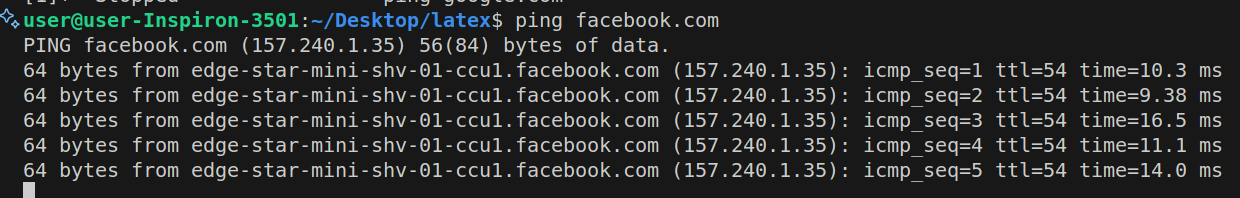
\includegraphics[width=0.8\textwidth]{ping.png}\par\vspace{1cm}


\subsubsection*{Analysis}
In the sample output, the PING command sends ICMP (Internet Control Message Protocol) packets to the specified host (in this case, \texttt{google.com}) and receives responses. The output includes information such as the round-trip time (rtt) for each packet and overall statistics.

By analyzing the PING output, you can assess the network connectivity and performance to the specified destination.
 

\subsubsection*{Limiting the number of PING requests}
By default, the PING command sends an unlimited number of requests to the destination. To limit the number of requests, use the \texttt{-c} option:

\subsubsection*{Sample Output}
$
ping -c <num> <destinationHost>
$
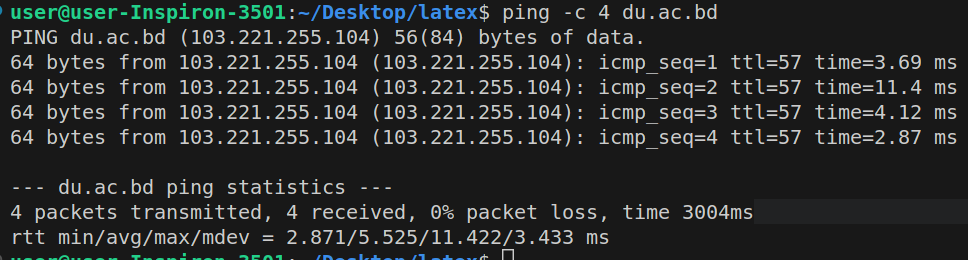
\includegraphics[width=0.8\textwidth]{pingCount.png}\par\vspace{1cm}

\subsubsection*{Analysis}
In the sample output, the PING command sends 4 ICMP packets to the specified host (in this case, \texttt{du.ac.bd}) and receives responses. The output includes information such as the round-trip time (rtt) for each packet and overall statistics.


\subsection{TRACEROUTE}
Using the {
    \texttt{traceroute}
} command, test the connectivity between two devices. When the traceroute is successful, record the RTT and the number of hops. When the traceroute is unsuccessful, record the error message. Repeat the test with different packet sizes and record the results.

\subsubsection*{Command Execution}
To use TRACEROUTE, open the terminal and execute the following command:
$traceroute <destinationHost>$
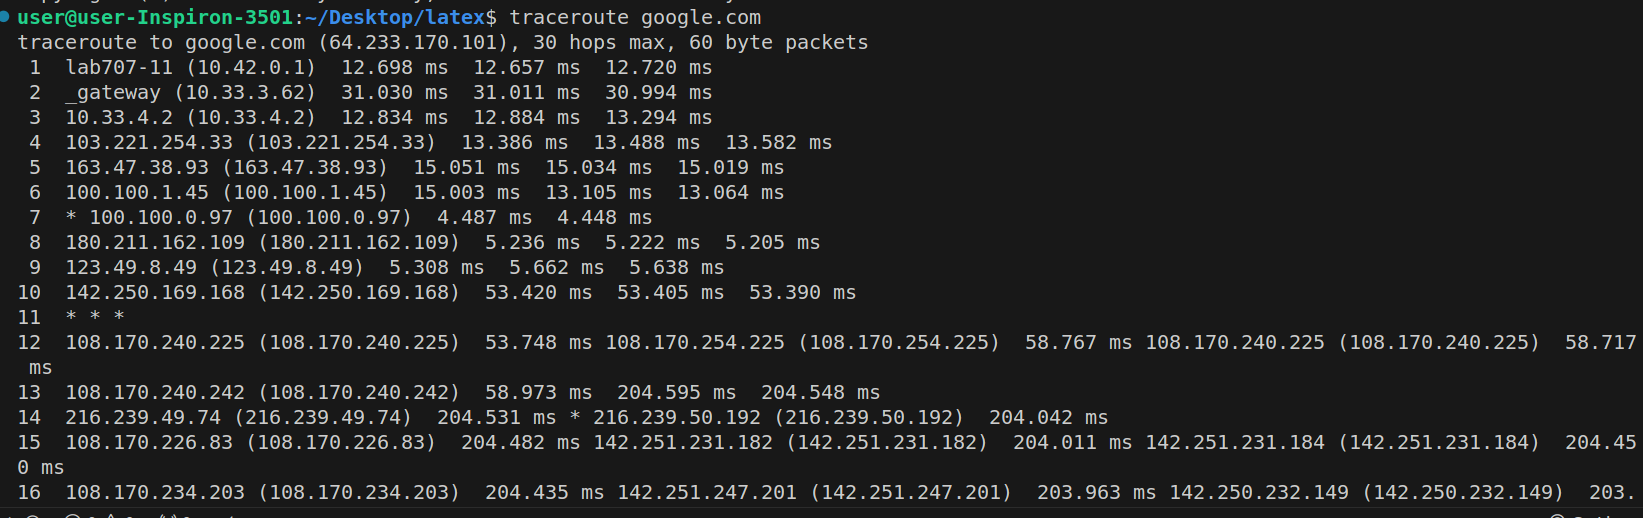
\includegraphics[width=0.8\textwidth]{traceroute.png}\par\vspace{1cm}
{\textbf{Number of hops}} is 30. It indicates the time to live (TTL) of the packet. The TTL value is decremented by one each time the packet is forwarded by a router. When the TTL value reaches zero, the packet is discarded and an ICMP error message is sent to the source. The source can use the ICMP error message to determine the IP address of the router that discarded the packet. The source can then use the IP address to determine the router name.

\subsubsection*{Limiting the number of hops}
By default, the TRACEROUTE command sends packets with a TTL value of 1 and increments the TTL value by 1 for each subsequent packet. To limit the number of hops, use the \texttt{-m} option:

\subsubsection*{Sample Output}
$
traceroute -m <num> <destinationHost>
$
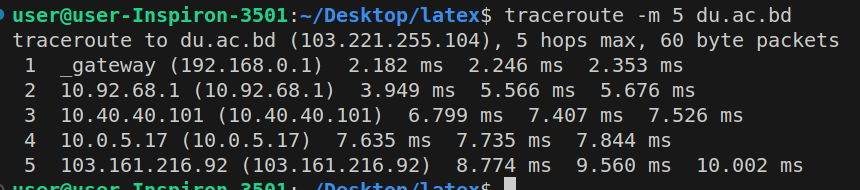
\includegraphics[width=0.8\textwidth]{tracerouteCount.png}\par\vspace{1cm}
We use 5 hops. It indicates the time to live (TTL) of the packet. The TTL value is decremented by one each time the packet is forwarded by a router. When the TTL value reaches zero, the packet is discarded and an ICMP error message is sent to the source. The source can use the ICMP error message to determine the IP address of the router that discarded the packet. The source can then use the IP address to determine the router name.

\subsection{IFCONFIG}
Using the {
    \texttt{ifconfig}
} command, display the IP address, subnet mask, and default gateway for a device. Record the results. The “{\textbf{ifconfig}}” command with no arguments will display all the active network interface configuration details that includes their assigned IP addresses, netmasks, and other relevant information.

\subsubsection*{Command Execution}
To use IFCONFIG, open the terminal and execute the following command:
$ifconfig$

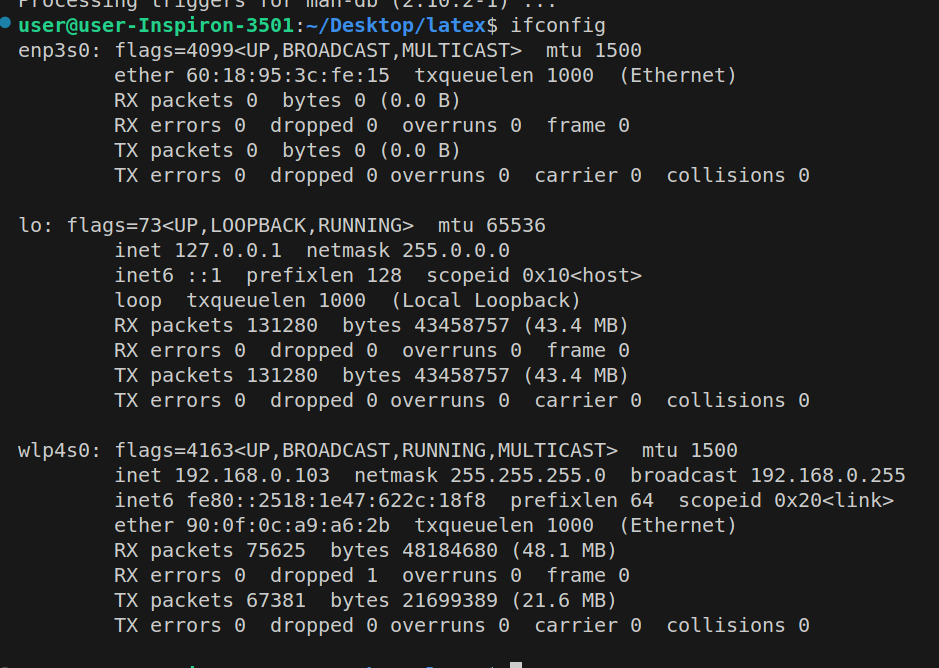
\includegraphics[width=0.8\textwidth]{ifconfig.png}\par\vspace{1cm}

\subsubsection*{Analysis}
In the sample output, the IFCONFIG command displays the IP address, subnet mask, and default gateway for the device. The output also includes information such as the MAC address, MTU, and the number of packets transmitted and received.

\subsubsection*{Disable a network interface}
To disable a network interface, use the \texttt{down} option:

\subsubsection*{Sample Output}
$
sudo ifconfig <interfaceName> down
$
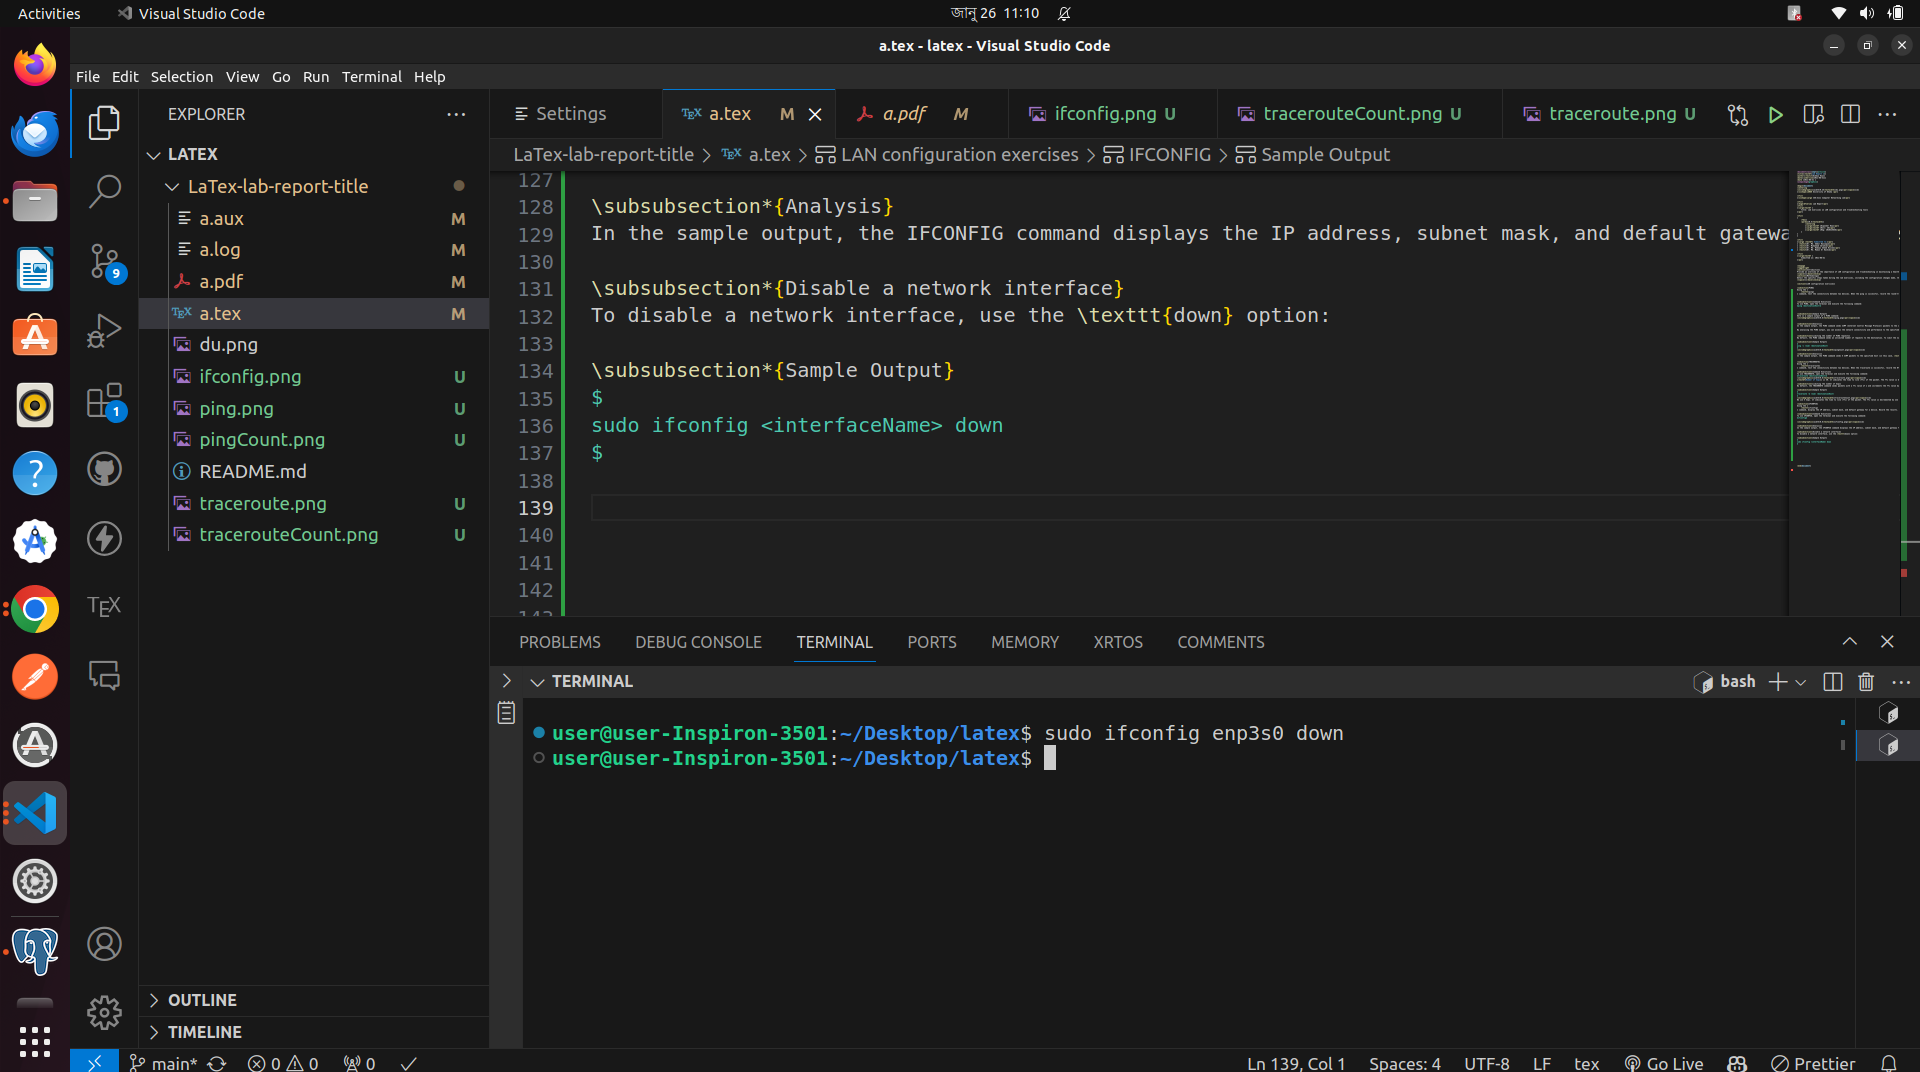
\includegraphics[width=0.8\textwidth]{ifconfigDown.png}\par\vspace{1cm}
The network interface is down.

\subsubsection*{Enable a network interface}
To enable a network interface, use the \texttt{up} option:

\subsubsection*{Sample Output}
$ sudo ifconfig <interfaceName> up $
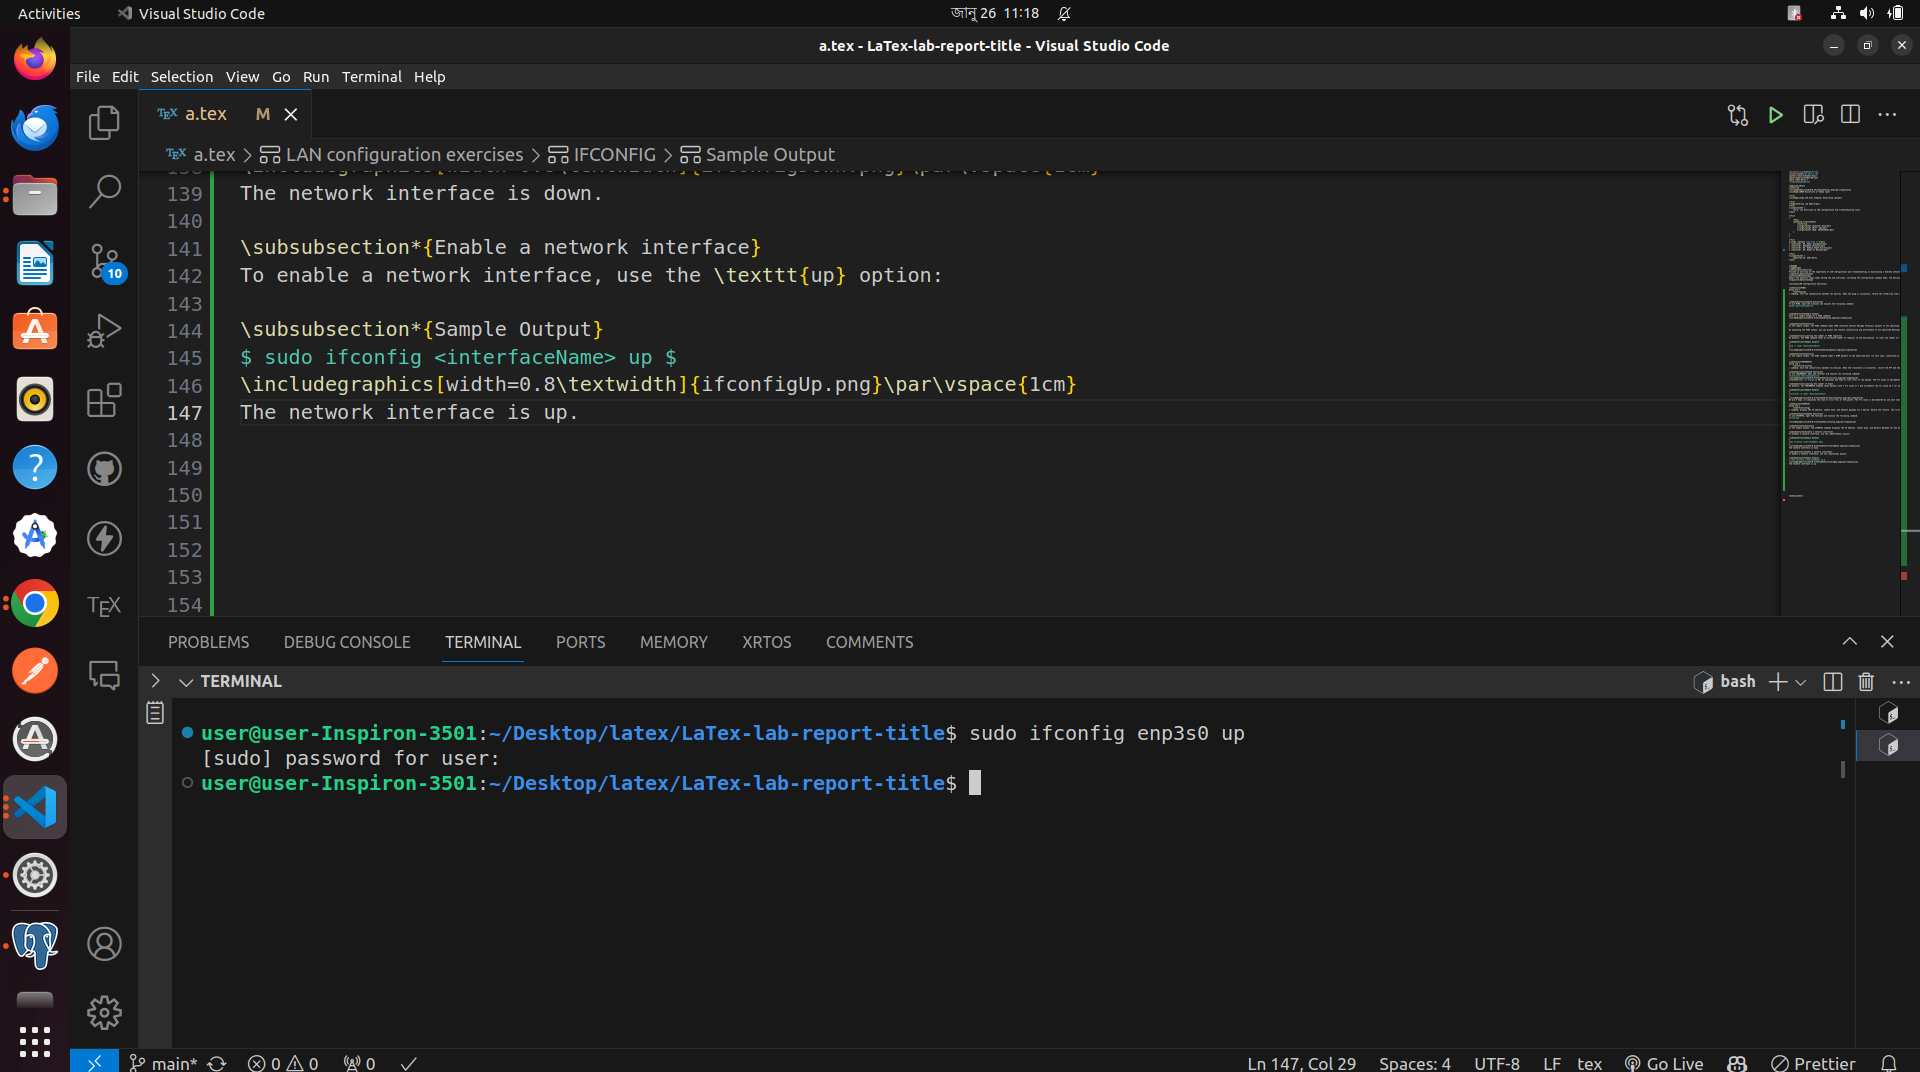
\includegraphics[width=0.8\textwidth]{ifconfigUp.png}\par\vspace{1cm}
The network interface is up.

\subsection{ARP}
Using the {
    \texttt{arp}
} command, display the ARP cache for a device. Record the results.

\subsubsection*{Command Execution}
To use ARP, open the terminal and execute the following command:
$arp$

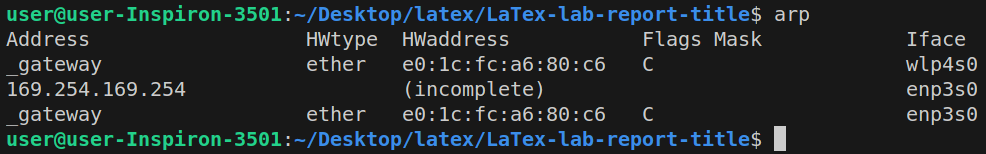
\includegraphics[width=0.8\textwidth]{arp.png}\par\vspace{1cm}

\subsubsection*{Analysis}
In the sample output, the ARP command displays the ARP cache for the device. The output includes information such as the IP address, MAC address, and type of each entry.

\subsection*{RARP}
Using the {
    \texttt{rarp}
} command, display the RARP cache for a device. Record the results.The Reverse Address Resolution Protocol (RARP) is a networking protocol that is used to map a physical (MAC) address to an Internet Protocol (IP) address. It is the reverse of the more commonly used Address Resolution Protocol (ARP), which maps an IP address to a MAC address.

\subsubsection*{Command Execution}
To use RARP, open the terminal and execute the following command:

$rarp$

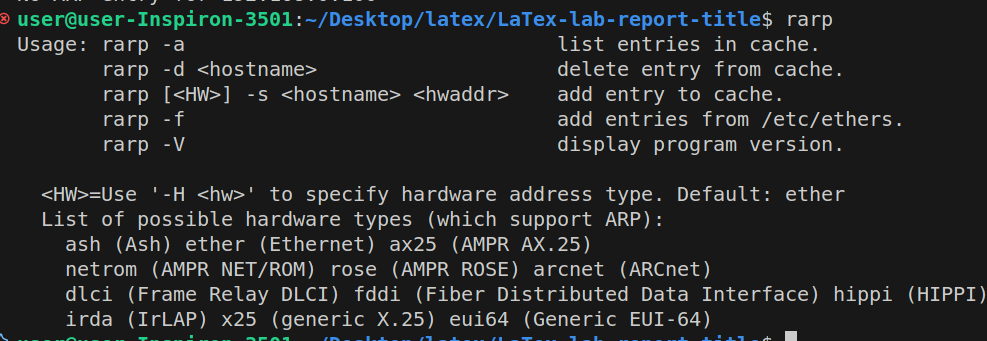
\includegraphics[width=0.8\textwidth]{rarp.png}\par\vspace{1cm}

\subsubsection*{Analysis}
In the sample output, the RARP command displays the RARP cache for the device. The output includes information such as the IP address, MAC address, and type of each entry.

\subsection*{NSLOOKUP}
Using the {
    \texttt{nslookup}
} command, display the DNS cache for a device. Record the results.

\subsubsection*{Command Execution}
To use NSLOOKUP, open the terminal and execute the following command:

$nslookup$

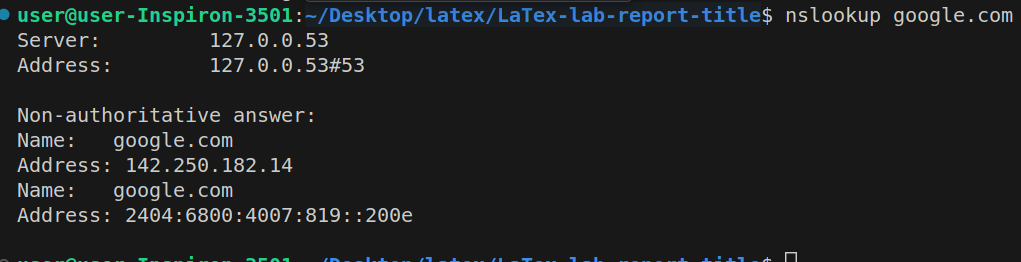
\includegraphics[width=0.8\textwidth]{nslookup.png}\par\vspace{1cm}

\subsubsection*{Analysis}
In the sample output, the NSLOOKUP command displays the DNS cache for the device. The output includes information such as the IP address, hostname, and type of each entry. nslookup followed by the domain name will display the “A Record” (IP Address) of the domain. Use this command to find the address record for a domain. It queries domain name servers and gets the details. 

\subsubsection*{Using type any}
To display all the information in the DNS cache, use the \texttt{set type=any} option:

\subsubsection*{Sample Output}
$nslookup -type=any <domainName>$

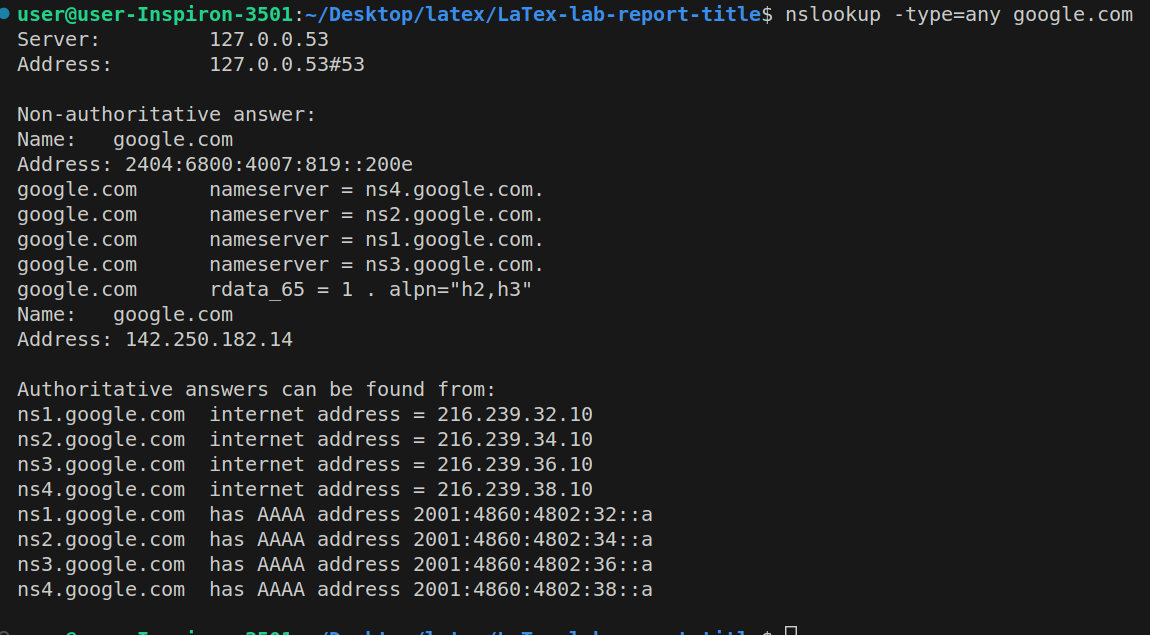
\includegraphics[width=0.8\textwidth]{nslookupAny.png}\par\vspace{1cm}


There are also available types of DNS records. The most common ones are:

\begin{itemize}
    \item A: Address record
    \item AAAA: IPv6 address record
    \item CNAME: Canonical name record
    \item MX: Mail exchange record
    \item NS: Name server record
    \item PTR: Pointer record
    \item SOA: Start of authority record
    \item TXT: Text record
\end{itemize}

\subsection*{NETSTAT}

Using the {
    \texttt{netstat}
} command, display the active TCP connections for a device. Record the results. The netstat command is like a special tool in Linux that helps you understand and check things about how your computer connects to the internet. It can tell you about the connections your computer is making, the paths it uses to send information, and even some technical details like how many packets of data are being sent or received. In simple terms, it’s like a window that shows you what’s happening with your computer and the internet. This article will help you learn how to use netstat, exploring different ways to get specific information and giving you a better idea of what’s going on behind the scenes.



\subsubsection*{Command Execution}

To use NETSTAT, open the terminal and execute the following command:


$netstat$

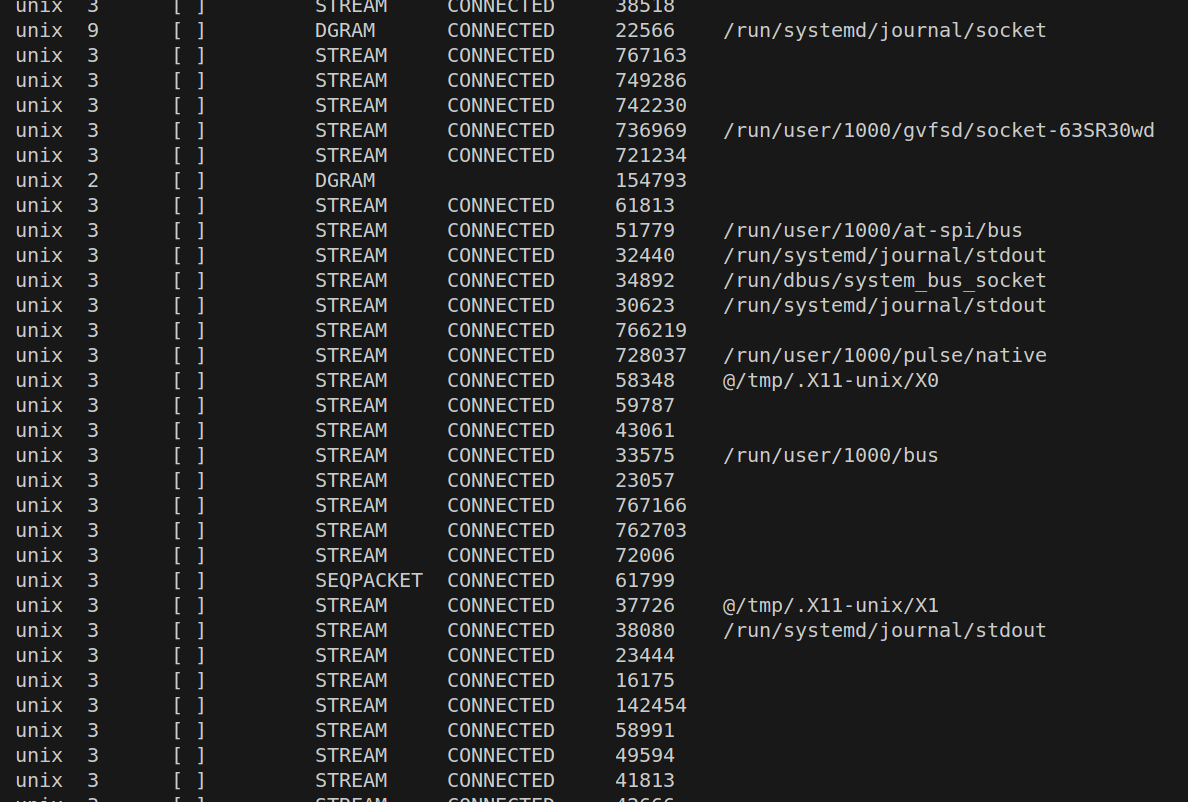
\includegraphics[width=0.8\textwidth]{netstat.png}\par\vspace{1cm}

\subsubsection*{Analysis}
In the sample output, the NETSTAT command displays the active TCP connections for the device. The output includes information such as the protocol, local address, foreign address, and state of each connection.

























\end{document}

